%%%%% Result and Discussion %%%%%
\section{Result and Discussion} 
\subsection{Error Analysis of Cross-Shaped Sheets}
At the early stage of the project, given that the number of cross-shape sheets in each modules may have an 
influence on the maximum bending angle $\boldsymbol{\alpha}_{max}$, which is an essential parameter of those which 
affect the range of working space of the manipulator, hence the number of sheets should be determined by deriving 
the functions of both absolute error and relative error \cite{fishboneCR} against the number of sheets. The 
simulation results are shown in Figure \ref{fig:error_analysis}.
\begin{figure}[H] %[H] "corresponds to start the figure Here" 
    \centering %alignment can be flushleft or flushright
    \captionsetup{labelsep=colon}
    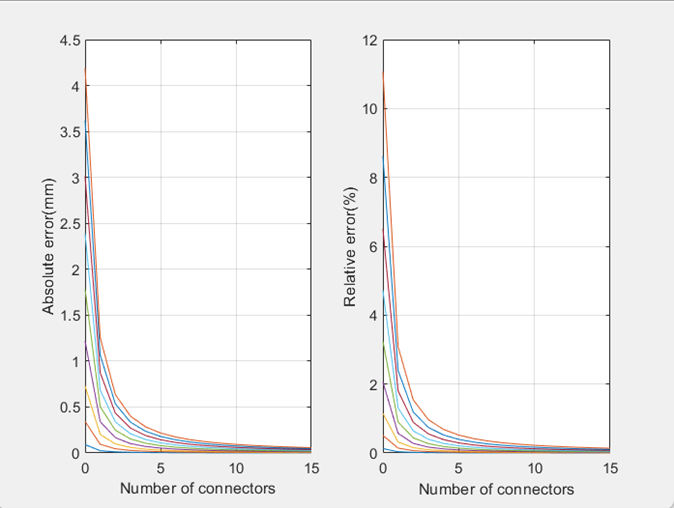
\includegraphics[width=0.75\textwidth]{Image/Result/error_analysis.png} 
    \caption[The simulation results of errors against the number of connecting sheets]
    {\centering \textbf{The simulation results of errors against the number of connecting sheets.}}
    \label{fig:error_analysis}
\end{figure}
As illustrated in graphs, the changing trends of both absolute and relative errors are almost identical since 
the relative error is proportional to the absolute error, and the different lines with different colors represent 
the data with different bending angles whose range is from 10 degrees to 90 degrees in both directions (positive 
or negative). It is obvious that both errors decrease with the increase in the number of connecting sheets, hence 
theoretically, the number of sheets should be as large as possible to make both errors could be negligible. However, 
the number of sheets also has an influence on the size of simulation space, more the number of sheets less the size 
of simulation space given that if the length of manipulator is much longer, the space near to the basement of 
manipulator could not be reached due to the characteristics of the material. Hence, the number of sheets could be 
assumed to be 10 rather than 15, even though both the errors are smaller when the number of sheets is 15. \\
\subsection{Workspace Analysis of Manipulator}
The simulation of workspace of the manipulator has been illustrated since it is important to determine the 
variables of joints based on the required workspace. The dimension of workspace is affected by several aspects, 
which include the simulation index and the parameter H representing the height of the basement of cubic in the 
original coordinate of the manipulator. The simulation results and the parameters are shown below.
\begin{figure}[H] %[H] "corresponds to start the figure Here" 
    \centering %alignment can be flushleft or flushright
    \captionsetup{labelsep=colon}
    \begin{subfigure}{0.45\textwidth} % subfigure 1
        \centering
        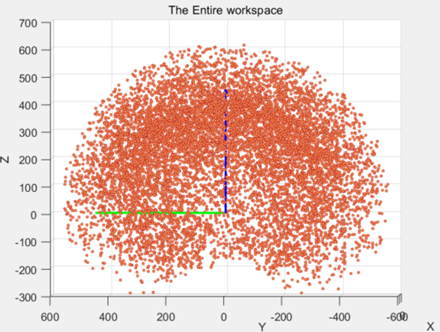
\includegraphics[width=\linewidth]{Image/Result/workspace_10000.png}
        \caption{\centering The entire workspace where simulation index=10000}
        \label{fig:ws_10000}
    \end{subfigure}
    \hfill
    \begin{subfigure}{0.45\textwidth} % subfigure 2
        \centering
        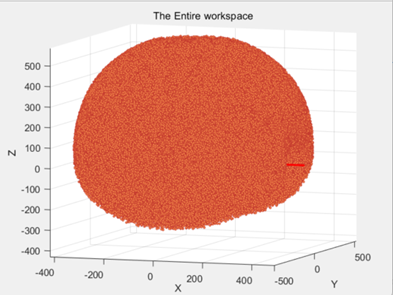
\includegraphics[width=\linewidth]{Image/Result/workspace_1000000.png}
        \caption{\centering The entire workspace where simulation index=1000000}
        \label{fig:ws_1000000}
    \end{subfigure}
    \caption[The entire workspace with different random indices]
    {\centering \textbf{The entire workspace with different simulation indices.}}
    \label{fig:ws_diff}
\end{figure}
\noindent As shown in Figure \ref{fig:ws_10000}, the working space of manipulator forms a spherical shell-shaped point 
cloud consisting of 10000 floating points since the simulation index is 10000, which is insufficient to fully 
occupied the theoretical workspace. To further generalize the theoretical workspace, it is necessary to enhance 
the simulation index. The appropriate workspace should be divided from the workspace. 
\begin{figure}[H] %[H] "corresponds to start the figure Here" 
    \centering %alignment can be flushleft or flushright
    \captionsetup{labelsep=colon}
    \begin{subfigure}{0.45\textwidth} % subfigure 1
        \centering
        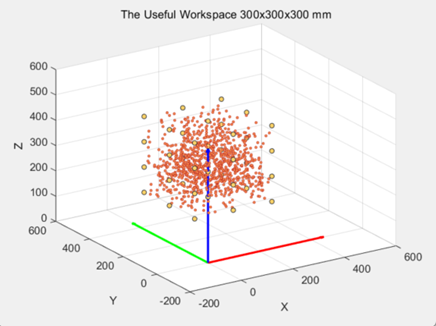
\includegraphics[width=\linewidth]{Image/Result/rect_workspace_10000_260-560.png}
        \caption{\centering The cubic workspace of manipulator with index = 10000 H=260-560mm}
        \label{fig:ws_10000_260}
    \end{subfigure}
    \hfill
    \begin{subfigure}{0.45\textwidth} % subfigure 2
        \centering
        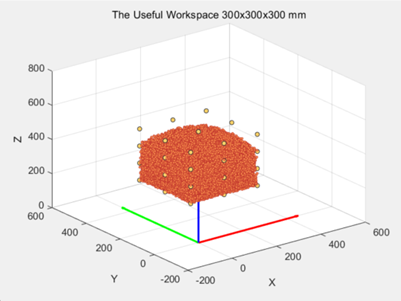
\includegraphics[width=\linewidth]{Image/Result/rect_workspace_1000000_350-650.png}
        \caption{\centering The cubic workspace of manipulator with index = 1000000 H=350-650mm}
        \label{fig:ws_1000000_350}
    \end{subfigure}
    \caption[The entire workspace with different random indices]
    {\centering \textbf{The cubic workspace with different simulation indices and different segmentation.}}
    \label{fig:ws_diff_segmentation}
\end{figure}
\noindent According to Figure \ref{fig:ws_diff_segmentation}, due to the limitation in the dimension of entire workspace, 
the upper part of the cubic space could not be fully occupied, in other words, is almost empty when H=350mm, which 
means that not all the points shown in yellow could be reached by the manipulator. Aiming to determine the ‘bond’ 
value of parameter H, the function of calculating the distance between the points in yellow in the same layer and 
the nearest floating points has been carried out and the simulation results with index=1000000 and H=300mm are 
shown below.
\begin{figure}[H] %[H] "corresponds to start the figure Here" 
    \centering %alignment can be flushleft or flushright
    \captionsetup{labelsep=colon}
    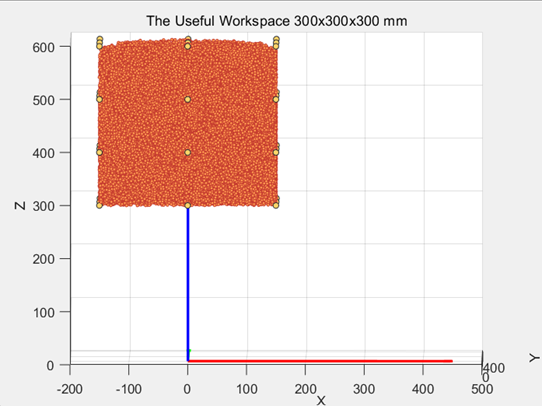
\includegraphics[width=0.75\textwidth]{Image/Result/rect_workspace_1000000_300-600.png} 
    \caption[The cubic workspace in X-Z plane with H=300mm]
    {\centering \textbf{The cubic workspace in X-Z plane with H=300mm.}}
    \label{fig:cub_ws_300_600}
\end{figure}
\noindent As shown in Figure \ref{fig:cub_ws_300_600}, almost the entire cubic workspace has been occupied by the floating 
points which indicates that the value of H could be considered as 300mm, but it is not rigor to concluded that the 
‘bond’ value is 300. The detailed data which shows the distance from the floating points to the nearest point which 
sits on the edge for each layer is shown below with the unit ‘mm’.
\begin{figure}[H] %[H] "corresponds to start the figure Here" 
    \centering %alignment can be flushleft or flushright
    \captionsetup{labelsep=colon}
    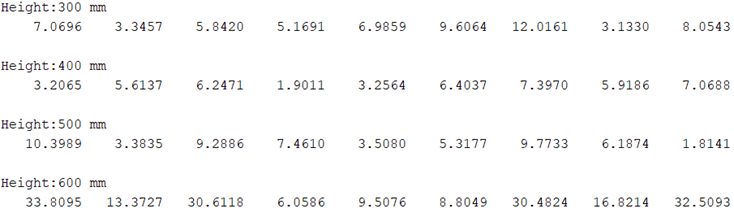
\includegraphics[width=0.9\textwidth]{Image/Result/distance_1000000_300-600.png} 
    \caption[The distance between random points and the nearest points on the edge with H=300mm]
    {\centering \textbf{The distance between random points and the nearest points on the edge with H=300mm.}}
    \label{fig:data_300_600}
\end{figure}
\noindent Before analyzing these data, the following top-down view of the cubic workspace will help to link each 
numerical value with the designated points.
\begin{figure}[H] %[H] "corresponds to start the figure Here" 
    \centering %alignment can be flushleft or flushright
    \captionsetup{labelsep=colon}
    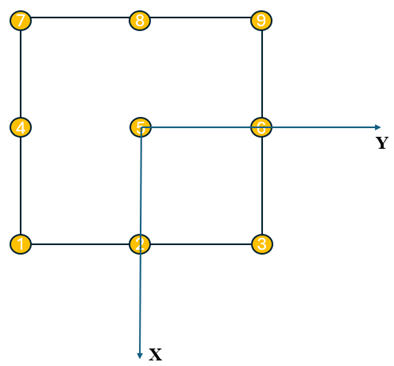
\includegraphics[width=0.6\textwidth]{Image/Result/top-down_view_rect_workspace.png} 
    \caption[The top-down view of the cubic workspace]
    {\centering \textbf{The top-down view of the cubic workspace.}}
    \label{fig:top_down_view}
\end{figure}
The first layer is the one with height of 300mm and the fourth layer is the one with height of 600mm, and the first 
thing should be check is the average distance between the random points and the nearest ‘edge’ point of layer two 
and layer three given that if the 18 points of these two layers could not be fully surrounded by the entire 
workspace, then those laying on the layer one and four couldn’t be reached by the end-effector as well. The average 
distance for layer 2 and 3 could be obtained by the following calculation.
\begin{align}
    d_{ave,300mm}=\frac{\sum_2^3 d}{18} = 5.7859mm
\end{align}
where 2 and 3 indicate the values of distance listed in the second and third row in Figure \ref{fig:data_300_600} 
and denominator means there are 18 points in two layers in total. Based on the value shown in row one and row four, 
the following table could be developed.
\begin{center}
    \small
    \begin{longtable}{l l l l l l l l l l}
    \caption{The Parameters of Manipulators.} \label{tab:distance_300_600} \\
    \hline \multicolumn{1}{l}{\textbf{Number}} & 
    \multicolumn{1}{l}{\textbf{1}} & 
    \multicolumn{1}{l}{\textbf{2}} & 
    \multicolumn{1}{l}{\textbf{3}} & 
    \multicolumn{1}{l}{\textbf{4}} & 
    \multicolumn{1}{l}{\textbf{5}} & 
    \multicolumn{1}{l}{\textbf{6}} &
    \multicolumn{1}{l}{\textbf{7}} & 
    \multicolumn{1}{l}{\textbf{8}} & 
    \multicolumn{1}{l}{\textbf{9}} \\ \hline 
    \endfirsthead
    \multicolumn{10}{c}%
    {{\bfseries \tablename\ \thetable{} -- continued from previous page}} \\
    \hline \multicolumn{1}{l}{\textbf{Number}} & 
    \multicolumn{1}{l}{\textbf{1}} & 
    \multicolumn{1}{l}{\textbf{2}} & 
    \multicolumn{1}{l}{\textbf{3}} & 
    \multicolumn{1}{l}{\textbf{4}} & 
    \multicolumn{1}{l}{\textbf{5}} & 
    \multicolumn{1}{l}{\textbf{6}} &
    \multicolumn{1}{l}{\textbf{7}} & 
    \multicolumn{1}{l}{\textbf{8}} & 
    \multicolumn{1}{l}{\textbf{9}} \\ \hline 
    \endhead
    \hline \multicolumn{10}{|r|}{{Continued on next page}} \\ \hline
    \endfoot
    \hline \hline
    \endlastfoot
    % table context
    \textbf{Layer 1} & 7.07 & 3.35 & 5.84 &	5.17 &	6.99 &	9.61 &	12.02 &	3.13 &	8.05 \\
    \textbf{Layer 4} &	33.81 &	13.37 &	30.61 &	6.06 &	9.51 &	8.81 &	30.48 &	16.82 &	32.51 \\
    \hline
    % \multirow{2}{*}{3D cartesian/gantry manipulator} & PPP & 3 & 1   \\
    % & & & \\ \hline
    \end{longtable}
\end{center}
Given that the average distance is 5.79mm, hence if the distance obtained in layer 1 and 4 is larger than the 
average one, it means that the end-effector could not reach that point. From the table and the calculated average 
distance in layer 2 and 3, the following points could be drawn.
\begin{itemize}
    \item Except No.2, No.4, No.8, all other points in both layers could not be reached by the end-effector since the distance is larger than the average value.
    \item The value of parameter H for this case is not suitable since almost all the ‘edge’ points on layer 1 and layer 4 could not be reached by the end-effector.
\end{itemize}
Hence, other values of H should be taken and compare the results with those with H=300mm. In this case, the value of 
H is taken as 280mm, and the simulation results are shown below.
\begin{figure}[H] %[H] "corresponds to start the figure Here" 
    \centering %alignment can be flushleft or flushright
    \captionsetup{labelsep=colon}
    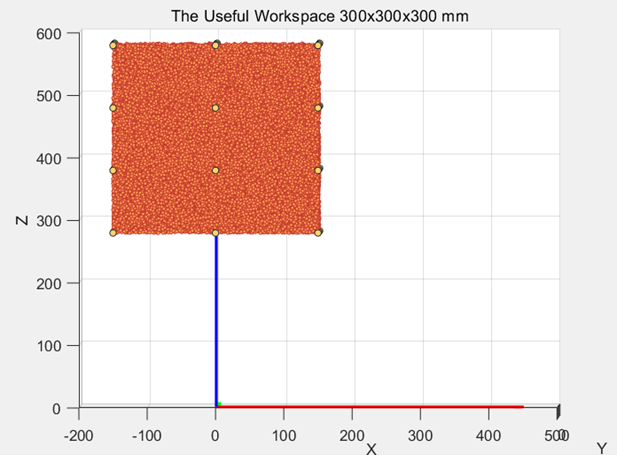
\includegraphics[width=0.6\textwidth]{Image/Result/rect_workspace_1000000_280-580.png} 
    \caption[The cubic workspace with index=1000000, H=280mm]
    {\centering \textbf{The cubic workspace with index=1000000, H=280mm.}}
    \label{fig:rect_ws_280_580}
\end{figure}
\begin{center}
    \small
    \begin{longtable}{l l l l l }
    \caption{The Parameters of Manipulators.} \label{tab:total_reachable} \\
    \hline \multicolumn{1}{l}{\textbf{H (mm)}} & 
    \multicolumn{1}{l}{\textbf{240}} & 
    \multicolumn{1}{l}{\textbf{260}} & 
    \multicolumn{1}{l}{\textbf{280}} & 
    \multicolumn{1}{l}{\textbf{300}} \\ \hline 
    \endfirsthead
    \multicolumn{5}{c}%
    {{\bfseries \tablename\ \thetable{} -- continued from previous page}} \\
    \hline \multicolumn{1}{l}{\textbf{H (mm)}} & 
    \multicolumn{1}{l}{\textbf{240}} & 
    \multicolumn{1}{l}{\textbf{260}} & 
    \multicolumn{1}{l}{\textbf{280}} & 
    \multicolumn{1}{l}{\textbf{300}} \\ \hline 
    \endhead
    \hline \multicolumn{5}{|r|}{{Continued on next page}} \\ \hline
    \endfoot
    \hline \hline
    \endlastfoot
    % table context
    Average distance (mm)	& 5.35	& 5.37	& 4.875	& 5.7859 \\
    Number of points could be reached in layer 1 and 4 & 1 & 4 & 5 & 3 \\
    \hline
    % \multirow{2}{*}{3D cartesian/gantry manipulator} & PPP & 3 & 1   \\
    % & & & \\ \hline
    \end{longtable}
\end{center}
Based on Table \ref{tab:total_reachable}, the suitable value of parameter H, the ‘bond’ height of the cubic, could be set to 280mm since the number of points could be reached in layer 1 and 4 is 5 which is more ideal than other cases. However, there are still some limitations in deciding the value of H which are shown below.
\begin{itemize}
    \item The value of the index is a little bit small, which has an influence on the distance between the floating points and the nearest ‘edge’ points. Hence the value of H could not be as precis as possible.
    \item There are too few trials have been carried out leading to the value of H is not convinced by others, and one possible way to deal with it is that develop a mathematic model i.e., Normal distribution, to predict the bond value of H which is more convincible.
    \item he data were obtained from few aspects which may affect the accuracy of the final value of H.
\end{itemize}


\subsection{Inverse Kinematics} % Done by Zehao Ye
This section will demonstrate the singular posture solution and trajectory replication results of the inverse 
kinematics algorithm. A comprehensive analysis of its accuracy and computational speed will be conducted, along 
with a description of its advantages and limitations. To begin with, it is essential to note that using angles 
as input for the programme is feasible due to the relative complexity of specifying the $\textbf{O}_{target}$ 
and $\textbf{P}_{target}$, which involves a total of 12 parameters. Moreover, the targets are generated based 
on angles by forward kinematics algorithm during the test. In essence, there is no substantial distinction 
between inputting angles and inputting coordinates.
\subsubsection{Singular Posture Solution}
Firstly, the bending of individual modules was tested as the target for the inverse kinematics solution. The 
inverse kinematics algorithm was tested for different angles of bending for Module 1, 2, 3, and 4, and the 
specific results are presented in Table \ref{tab:single_posture_IK} in Appendix \ref{append:table}. The 
solutions about the Modules 3 and 4 are highly satisfactory, with Module 3 even converging to error of 0.02mm 
in 6 epochs. However, the bending results for Module 1 and 2 are unsatisfied, which is caused by inappropriate 
initialization. According to the flowchart in Figure \ref{fig:flowchart}, the FABRIKc algorithm requires an 
initialization to start iterations. Taking the example of the target with 
$\boldsymbol{\alpha} = [0,\ 90,\ 0,\ 0]\degree$, after initializing with the initial posture in Figure 
\ref{fig:kinematics model 0_0_0_0} and applying the FABRIKc algorithm for iterations, the first iteration yields 
a posture with 
$\boldsymbol{\theta} = [-0.0,\ 104.04,\ -0.0,\ -22.0]\degree$. Moreover, since each iteration starts from Module 4, the error 
in Module 4 cannot be eliminated and persists. To mitigate this effect, selecting a more suitable posture for 
initialization is crucial, which can be solved trajectory replication. If the posture used for initialization with 
$\boldsymbol{\alpha} = [0,\ 100,\ 0,\ 0]\degree$, the solution of inverse kinematics algorithm would be 
$\boldsymbol{\theta} = [-0.0,\ 81.77,\ -0.0,\ 9.3]\degree$. Nevertheless, due to errors generated by the iteration sequence, 
complete elimination remains challenging, and efforts are focused on minimizing them as much as possible. \\
Afterwards, the complex bending angles of modules was utilized to investigate the influences of initialization. 
The target with angles $\boldsymbol{\alpha} = [80,\ 120,\ -120,\ 90]\degree$ is selected because its solution is complex, and 
it lies within the workspace of manipulator. The posture of the manipulator is shown in Figure 
\ref{fig:complex_target}. This scenario is likely to occur in practical applications and necessitates resolution 
through relevant methods.
\begin{figure}[H] %[H] "corresponds to start the figure Here" 
    \centering %alignment can be flushleft or flushright
    \captionsetup{labelsep=colon}
    \begin{subfigure}{0.9\textwidth} % subfigure 1
        \centering
        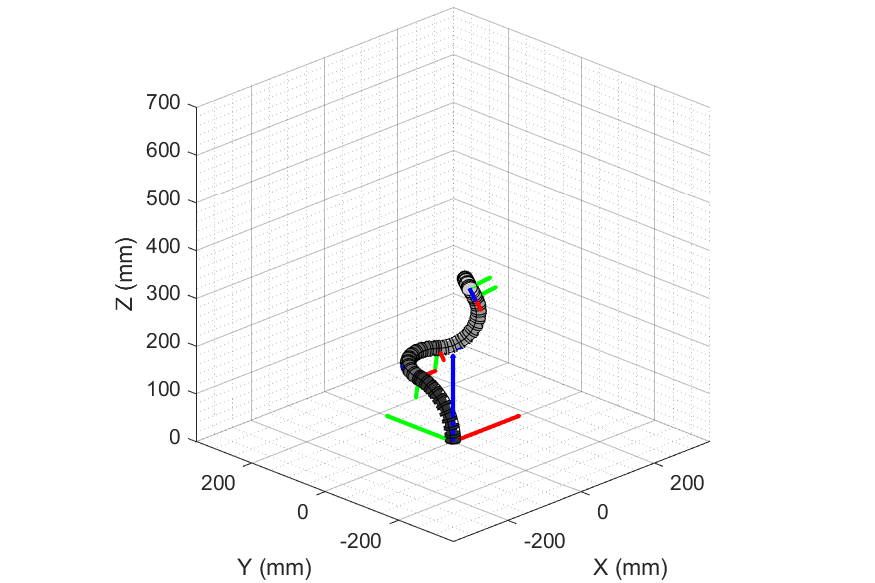
\includegraphics[width=\linewidth]{Image/MATLAB/manipulator_80_120_-120_90.png}
        \caption{\centering target: $\boldsymbol{\alpha} = [80,\ 120,\ -120,\ 90] \degree$ \\ \qquad}
        \label{fig:complex_target}
    \end{subfigure}
    \begin{subfigure}{0.45\textwidth} % subfigure 2
        \centering
        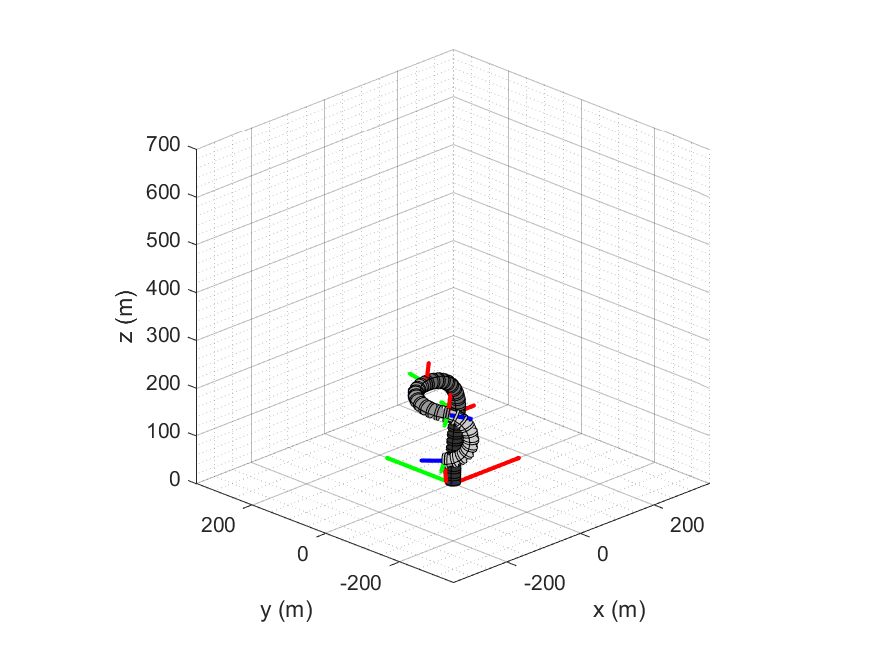
\includegraphics[width=\linewidth]{Image/MATLAB/manipulator_-8.88_-89.99_-126.81_-169.73.png}
        \caption{\centering initialization: $\boldsymbol{\alpha} = [0, 0, 0, 0]\degree$ \\
        $\boldsymbol{\theta} = [-8.88,\ -89.99,\ -126.81,\ -169.73]\degree$ }
        \label{fig:complex_init_0_0_0_0}
    \end{subfigure}
    \begin{subfigure}{0.45\textwidth} % subfigure 3
        \centering
        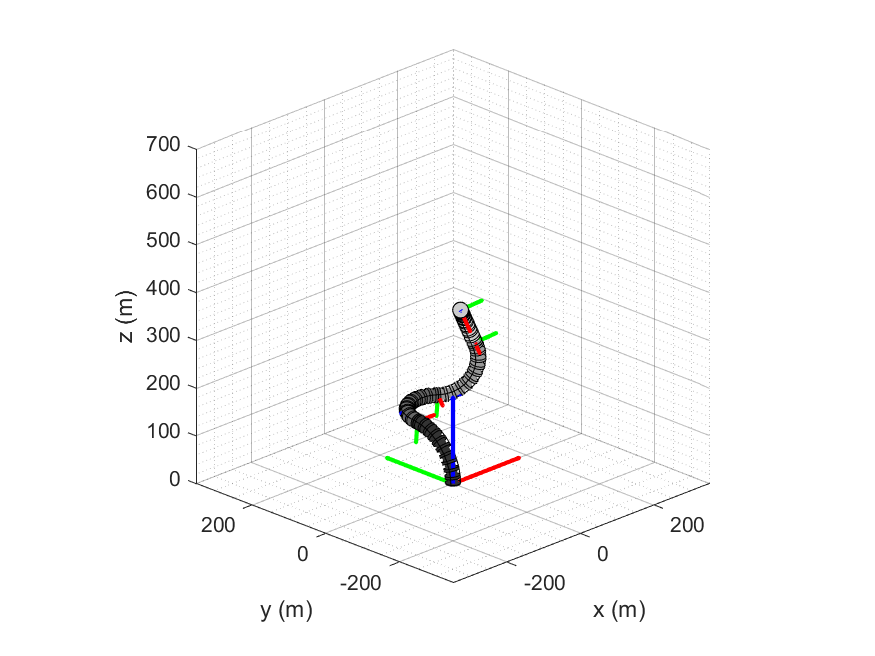
\includegraphics[width=\linewidth]{Image/MATLAB/manipulator_84.98_122.93_-114.9_63.01.png}
        \caption{\centering initialization: $\boldsymbol{\alpha} = [85, 125, -115, 55]\degree$ \\
        $\boldsymbol{\theta} = [84.98,\ 122.93,\ -114.9,\ 63.01]\degree$ }
        \label{fig:complex_init_85_125_-115_55}
    \end{subfigure}
    \caption[The kinematics model of manipulator with respective bending modules]
    {\centering \textbf{The inverse kinematics algorithm with different initialization.}}
    \label{fig:80_120_-120_90_diff_initial}
\end{figure}
\noindent With the initialization using the initial posture, the solution is 
$\boldsymbol{\theta} = [-8.88, -89.99, -126.81, -169.73]\degree$, which is shown in Figure \ref{fig:complex_init_0_0_0_0}. 
However, the solution of inverse kinematics algorithm would be $\boldsymbol{\theta} = [84.98,\ 122.93,\ -114.9,\ 63.01]\degree$, 
which is significantly close to the target while the angles for initialization are $[85,\ 125,\ -115,\ 55]\degree$. 
The solution of the inverse kinematics with more appropriate initialization is shown in Figure 
\ref{fig:complex_init_85_125_-115_55}. This signifies that if the manipulator is presently in a posture similar 
to the target configuration, it can accurately determine the corresponding bending angles $\boldsymbol{\theta}$ through the 
inverse kinematics algorithm. This proves to be highly beneficial for trajectory replication. \\
Ultimately, The efficient computational capability of algorithm is one of its strengths. The algorithm only 
takes 1.905 seconds to complete 10,000 epochs updating. In practical applications, it requires only 200 epochs 
to determine convergence. In comparison to traditional methods like inverse Jacobian \cite{inverse_jacobian}, 
which involve matrix transformations and derivatives, this approach can provide potential solutions in a short 
time, addressing the issue of singular points. However, this method has its limitations. In scenarios with 
multiple segments, the algorithm may introduce significant errors due to the calculation order, and these errors 
can be challenging to eliminate. The only viable solution is to enhance the algorithm's performance through 
careful initialization methods.
\subsubsection{Trajectory Replication}
The preceding discussion has highlighted the use of the current posture for initialization in trajectory 
replication. In this phase, two types of trajectories were replicated: arc segments and closed paths. This 
section will analyze these two trajectories, elucidating the strengths and weaknesses of inverse kinematics 
algorithm. \\
\begin{figure}[H] %[H] "corresponds to start the figure Here" 
    \centering %alignment can be flushleft or flushright
    \captionsetup{labelsep=colon}
    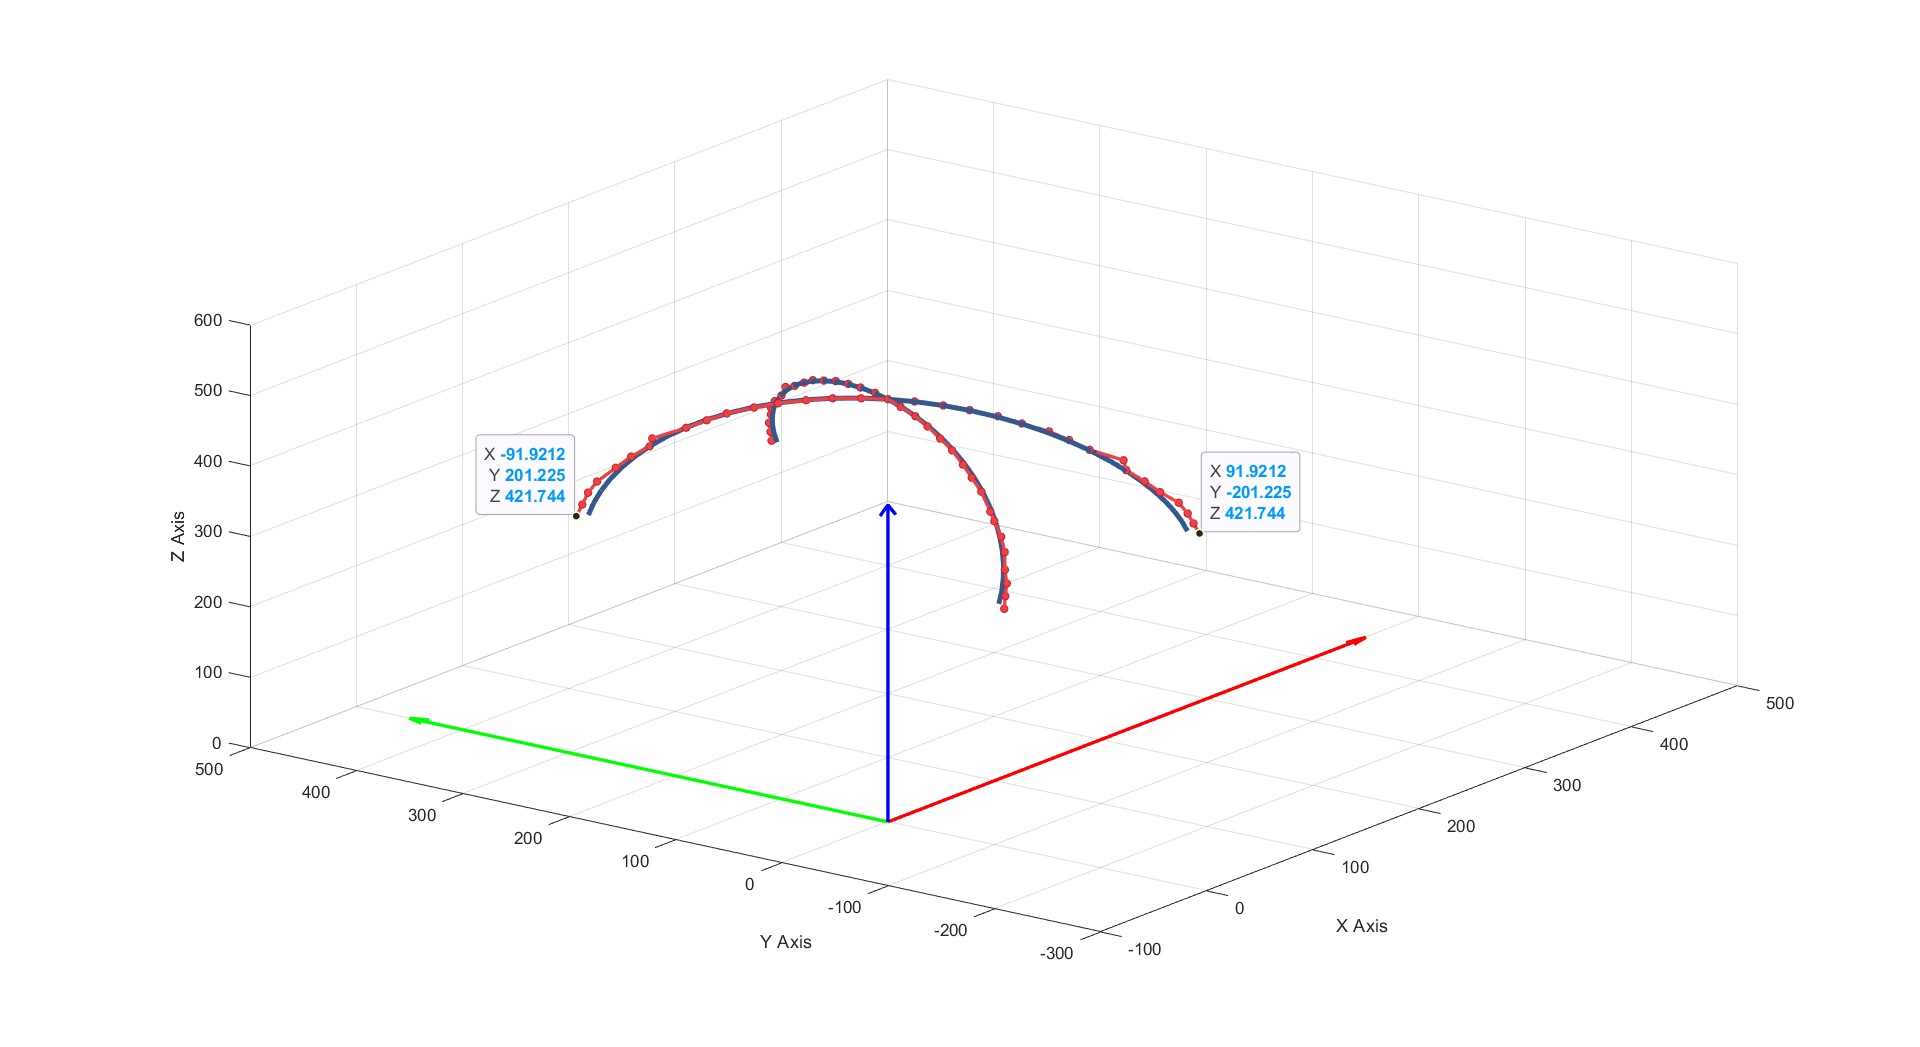
\includegraphics[width=1.0\textwidth]{Image/Result/cross_trajectory_replication_with_label.png} 
    \caption[The cross-shaped trajectory and its replication by FABRIKc algorithm]
    {\centering \textbf{The cross-shaped trajectory and its replication by FABRIKc algorithm.}}
    \label{fig:tr_cross}
\end{figure}
\begin{figure}[H] %[H] "corresponds to start the figure Here" 
    \centering %alignment can be flushleft or flushright
    \captionsetup{labelsep=colon}
    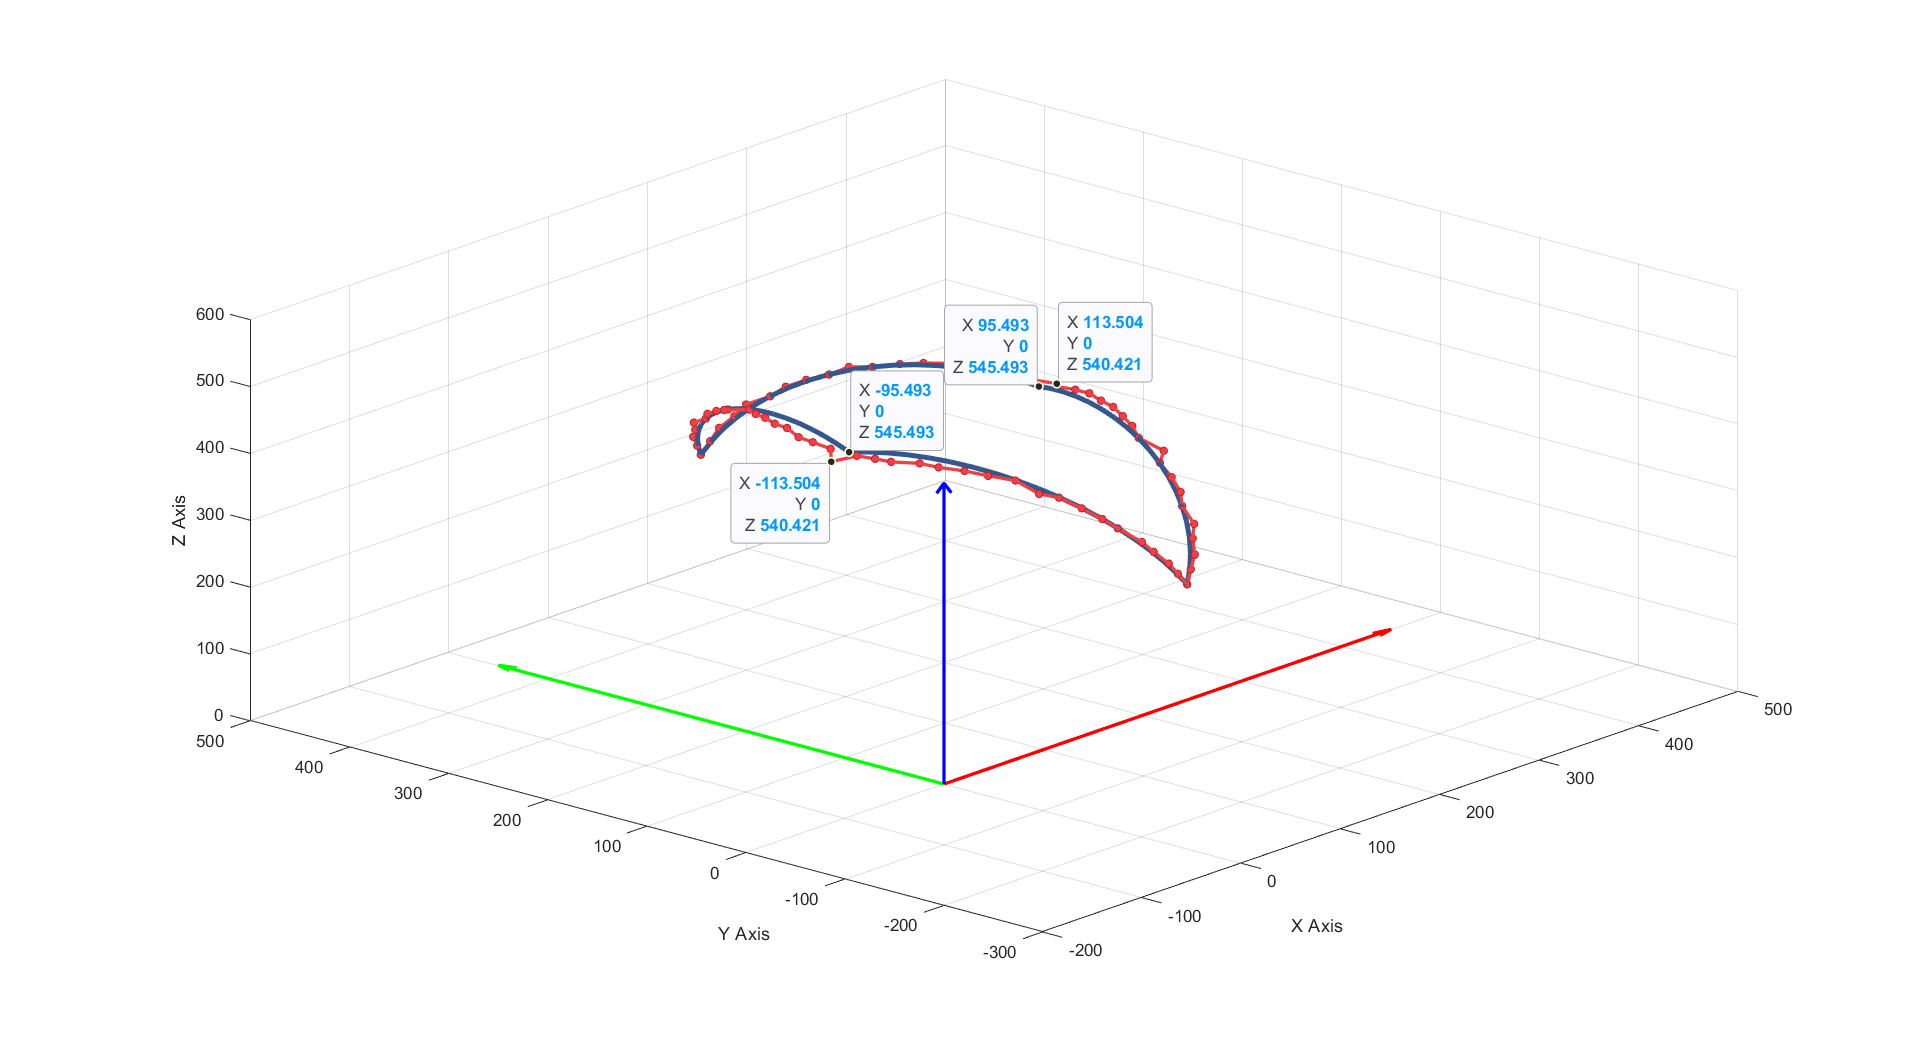
\includegraphics[width=1.0\textwidth]{Image/Result/circle_trajectory_replication_with_label.png} 
    \caption[The closed trajectory and its replication by FABRIKc algorithm]
    {\centering \textbf{The closed trajectory and its replication by FABRIKc algorithm.}}
    \label{fig:clc_cross}
\end{figure}
\textcolor{red}{TODO: make analysis about this part, calculate the error}

\subsubsection{The improvement about Inverse kinematics algorithm}
\textcolor{red}{TODO:talking about improvement to do about inverse kinematics, which are more detailed control method}

\subsection{Electroinc Control}
Initially, the testing of the results was supposed to be carried out through Proteus simulation. However, 
it was discovered that during the simulation process in Proteus, the motor components did not function normally, 
with frequent occurrences of stepping errors. At the same time, the simulation couldn't be completed in real-time 
due to the heavy load on the computer CPU. After consideration, the team members purchased a complete set of real 
components for testing. In the real circuit, the pin that each motor occupies are listed in the table below to 
reduce the complexity of wiring: \\

Connect the components as shown in the figure below, and run the program. \\
\\
Once started, the first thing the user needs to do is to input the values of $\Delta S_1 \sim \Delta S_8$: \\
\\
From the graph above we can see that$\Delta S_1 \sim \Delta S_8$ is:\\ 0mm, 0mm, -8mm, 8mm, -15mm, 15mm, 65mm, 
-65mm.\\ The value of $\Delta S_i$ is always in pairs, e.g, two cables controlling the same unit should always have 
the opposite $\Delta S_i$ value, this is decided by the working principle of the manipulator. \\
After conversion, the corresponding $Step_1 \sim Step_8$ should be: \\0, 0, -521, 521, -978, 978, 4237, -4237. 
(“-” sign represents counterclockwise steps). \\
Wait for the motors to finish stepping, once it's done, use function \emph{Serial.print(motor.currentPosition())} to 
check if the motors stepped correctly: \\
\\
As Figure above shows, all the motors are working correctly. In this program, all floating-point precision 
is taken to the last four decimal places (but the result printed on the monitor only shows two decimal places), 
so the accuracy of the result is beyond acceptable (from the above figure, maximum 0.01mm error).\\
Then, reset the motors, the motors went back to initial condition, which is $Step_1 \sim Step_8=0$. Repeat the 
motor stepping process, but this time, the motors are starting from a previous location from\\0mm, 0mm, -8mm, 
8mm, -15mm, 15mm, 65mm, -65mm to\\33mm, -33mm, 16mm, -16mm, 0mm, 0mm, 10mm, -10mm.\\
The difference $\Delta S_i - Delta S_i(prev)$ is: \\
33mm, -33mm, 24mm, -24mm, 15mm, -15mm, -55mm, 55mm.\\
The steps for motors are: 2151, -2151, 1565, -1565, 978, -978, -3585, 3585 steps.\\
Verify the result again by checking how many revolutions each motors rotated:\\
\\
The results are correct. Hence, the actuation control part runs correctly.
The program code is uploaded to Github: https://github.com/yezehao/Compact-Continuum-Manipulator-Platform/tree
/main/Arduino-Simulation


% \begin{figure}[H] %[H] "corresponds to start the figure Here" 
%     \centering %alignment can be flushleft or flushright
%     \captionsetup{labelsep=colon}
%     \begin{subfigure}{0.45\textwidth} % subfigure 1
%         \centering
%         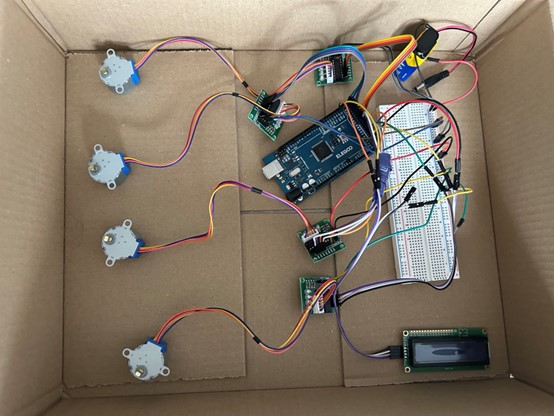
\includegraphics[width=\linewidth]{Image/Result/example.jpg}
%         \caption{\centering \textbf{Motor 1} - 0 steps, motor remains unchanged.}
%     \end{subfigure}
%     \hfill
%     \begin{subfigure}{0.45\textwidth} % subfigure 2
%         \centering
%         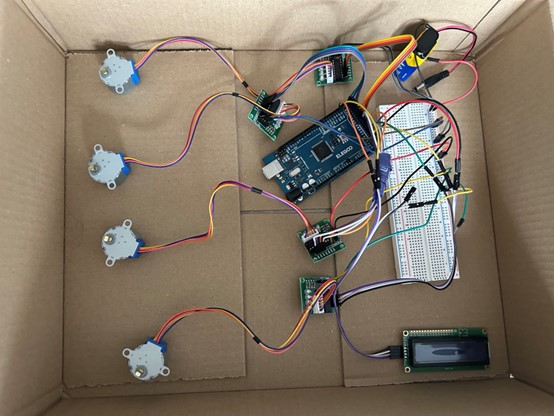
\includegraphics[width=\linewidth]{Image/Result/example.jpg}
%         \caption{\centering \textbf{Motor 2} - 0 steps, motor remains unchanged.}
%     \end{subfigure}
%     \begin{subfigure}{0.45\textwidth} % subfigure 3
%         \centering
%         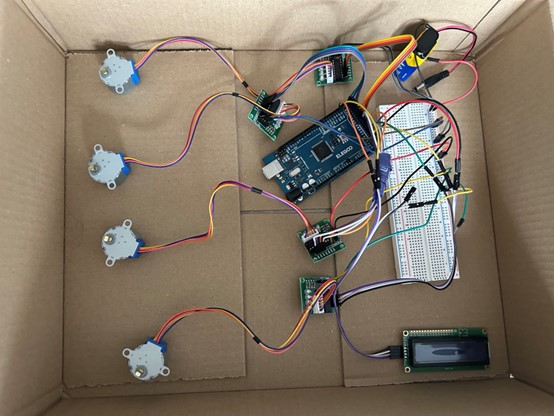
\includegraphics[width=\linewidth]{Image/Result/example.jpg}
%         \caption{\centering \textbf{Motor 3} - -521 steps/2048 steps=-0.255 rev.}
%     \end{subfigure}
%     \hfill
%     \begin{subfigure}{0.45\textwidth} % subfigure 4
%         \centering
%         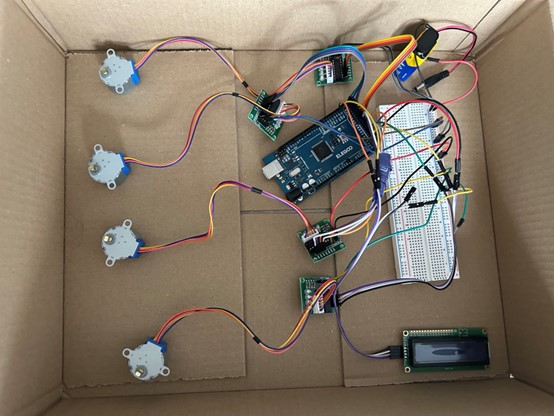
\includegraphics[width=\linewidth]{Image/Result/example.jpg}
%         \caption{\centering \textbf{Motor 4} - 521 steps/2048 steps = 0.255 rev.}
%     \end{subfigure}
% \end{figure}
% As Figure \ref{fig:8motor_motions} shows above, all the motors are working correctly.
% Then, reset the motors, the motors went back to initial condition, which is $Step_1 \sim Step_8=0$.



% change to new page
\newpage